\documentclass[a4paper]{article}
\usepackage{graphicx}
\graphicspath{ {./img/} }


\begin{document}
\title{Computer Architecture Lab 1 Report}
\author{Fabian Wüthrich}
\date{Oktober 2020}
\maketitle

\noindent
TODO short intro

\section*{Benchmarks}

For the exploration of the cache simulator the programs in
\verb|inputs/benchmark| were used:
\begin{description}
    \item[\texttt{stream}] A 64KB array is written sequentially and read back afterwards
    \item[\texttt{locality}] Used to test temporal and spatial locality
    \item[\texttt{strided}] Strided access to a 64KB array
\end{description}
Each benchmark starts with a cold cache and the working set size is always 64KB.

\section*{Cache Parameters}

For each benchmark the following cache parameters were tested to measure IPC:
\begin{itemize}
    \item Cache size from 0 to 256KB (0 is without caching) with a block size of
        4 bytes and associativity 1
    \item Block size from 4 to 2048 bytes with fixed cache size of 32KB and associativity 1
    \item Associativity from 1 to 512 with cache size 32KB and block size 32 bytes
\end{itemize}
The differences between each benchmark are discussed for the rest of this section.

\subsection*{stream Benchmark}

TODO Explain Results

\begin{figure}
    \centering
    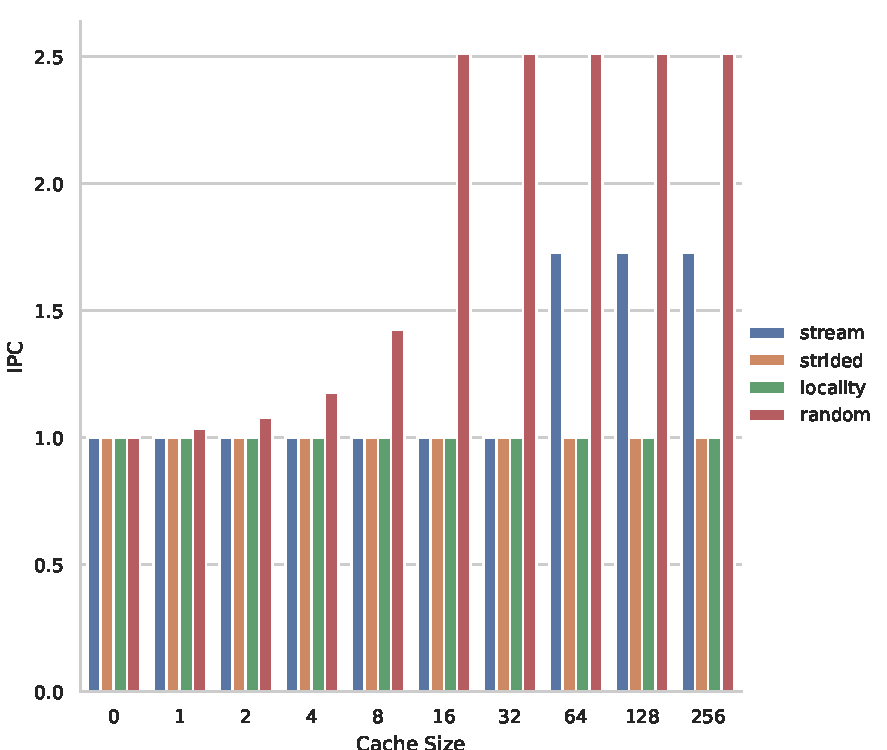
\includegraphics[width=\textwidth]{cache_size}
    \caption{Cache Size}
    \label{fig:cache-size}
\end{figure}

\begin{figure}
    \centering
    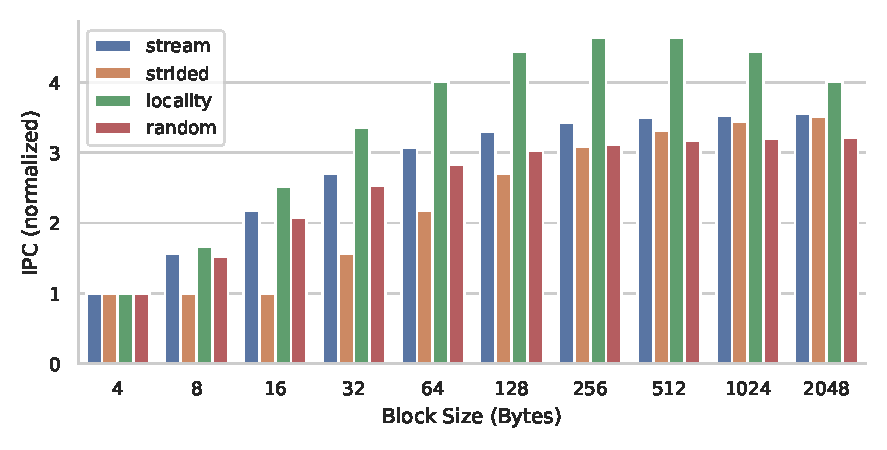
\includegraphics[width=\textwidth]{block_size}
    \caption{Block Size}
    \label{fig:block-size}
\end{figure}

\begin{figure}
    \centering
    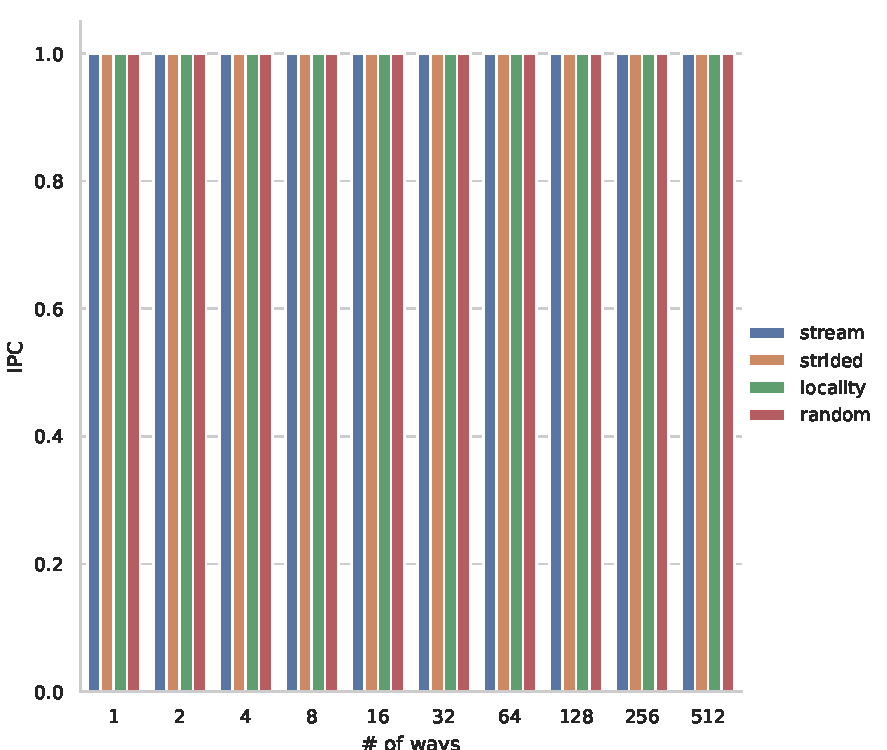
\includegraphics[width=\textwidth]{ways}
    \caption{Associativity}
    \label{fig:ways}
\end{figure}

\section*{Replacement/Insertion Policy}
TODO

\end{document}
